% flashcards-title: Two marked positions on a whole-number line
% flashcards-desc: A horizontal number line is labeled from zero through six. A is marked at two and B is marked at five.
\documentclass[dvisvgm,tikz,border=8pt]{standalone}
\usetikzlibrary{arrows.meta,patterns}

\definecolor{qraNavy}{HTML}{17324D}
\definecolor{qraBlue}{HTML}{2B6CB0}
\definecolor{qraGold}{HTML}{B7791F}
\definecolor{qraPale}{HTML}{EAF2F8}
\definecolor{qraGray}{HTML}{5C6773}

\tikzset{
  qra axis/.style={draw=qraNavy, line width=1.2pt},
  qra tick/.style={draw=qraNavy, line width=1pt},
  qra guide/.style={draw=qraGray, densely dashed, line width=0.8pt},
  qra counter/.style={circle, draw=qraNavy, fill=qraPale, line width=0.9pt, minimum size=7mm, inner sep=0pt},
  qra label/.style={font=\sffamily\bfseries, text=qraNavy},
  qra small label/.style={font=\sffamily, text=qraNavy},
}

\begin{document}
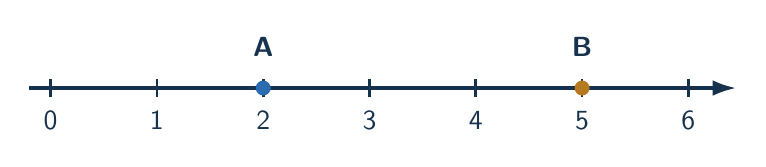
\begin{tikzpicture}[x=1.35cm,y=1cm]
  \draw[qra axis, -{Latex[length=3mm,width=2mm]}] (-0.2,0) -- (6.45,0);
  \foreach \x in {0,...,6} {
    \draw[qra tick] (\x,-0.12) -- (\x,0.12);
    \node[qra small label, below=5pt] at (\x,0) {\x};
  }
  \fill[qraBlue] (2,0) circle (2.7pt);
  \node[qra label, above=8pt] at (2,0) {A};
  \fill[qraGold] (5,0) circle (2.7pt);
  \node[qra label, above=8pt] at (5,0) {B};
\end{tikzpicture}
\end{document}
